\documentclass[11pt]{article}

\usepackage[margin=0.95in]{geometry}
\usepackage{microtype}
\usepackage{booktabs}
\usepackage{array}
\usepackage{tikz}
\usetikzlibrary{arrows.meta, positioning, fit, calc}
\usepackage{xcolor}
\usepackage{enumitem}
\usepackage[hidelinks]{hyperref}
\usepackage{caption}
\captionsetup{font=small, labelfont=bf}

\definecolor{ink}{HTML}{1D2129}
\definecolor{accent}{HTML}{1A5FB4}
\definecolor{warn}{HTML}{8A4600}
\definecolor{boxfill}{HTML}{E7F0FB}
\definecolor{stofill}{HTML}{FDF3E5}

\newcommand{\keep}[1]{\textcolor{accent}{\textbf{#1}}}

\title{\vspace{-1.2em}The Skateboard: a Minimum Framework for AI-Assisted\\ Porting of Fortran 2008 to GPU, with Professional Assurances\vspace{-0.4em}}
\author{Pared down from \texttt{answers.html}; three-month scope}
\date{July 23, 2026}

\setlength{\parskip}{0.35em}

\begin{document}
\maketitle
\vspace{-1.5em}

\section{Purpose and the claim being demonstrated}

The full framework in \texttt{answers.html} describes eleven components and fourteen requirements. It is the right design for a program that, like DARPA TRACTOR, must port many codes repeatedly. Our near-term goal is different: in three months, demonstrate on one 30{,}000-line Fortran 2008 code that an AI agent can carry out GPU ports \emph{with little human intervention}, and that the result is \emph{correct}, \emph{effective}, and \emph{repeatable} to a standard an engineering organization would accept. This document specifies the least framework that supports that claim --- the skateboard, in the sense of the smallest artifact that rolls end to end, rather than a wheel from the eventual car.

The paring rule is simple, and it comes straight from the TRACTOR evidence. Every component in the full design does one of two things: it \emph{produces evidence} for a claim (correct, effective, repeatable), or it \emph{improves throughput and scale} (planners, ensembles, provenance graphs, compiler matrices, prompt optimization). We keep everything in the first category, essentially intact, because the assurances are the demonstration. We cut or manually substitute everything in the second category, because with one code, a handful of candidate regions, and three months, a human can do those jobs in hours. The demonstration loses nothing it needs: TRACTOR's central finding is that outcomes are driven by orchestration and oracles, not by generation --- and oracles are precisely what we are keeping.

This framing also serves the client story about how professional AI use differs from personal AI use. The agent is the same in both settings. What differs is the harness: a developer on a personal project accepts ``the tests I remembered to run passed on my machine,'' while an engineering organization requires oracles the agent cannot edit, gates that make forbidden outcomes impossible, and a record that lets a reviewer reconstruct why each change was accepted. The skateboard \emph{is} that harness, at minimum size; the demo makes the difference visible by construction.

\section{What survives the cut}

Four things are kept whole. Each maps to one of the three claims.

\textbf{1. The correctness oracle: capture-replay tests plus a tolerance comparator (claim: correct).}
We instrument each candidate region during runs on representative datasets, capture every input the region reads and every output it writes (arguments, module variables, any residual \texttt{COMMON} state), and generate a standalone replay driver. A comparator checks replayed outputs against captured outputs under per-quantity tolerances --- absolute, relative, or units-in-the-last-place --- because a GPU port legitimately changes floating-point results (fused multiply-add contraction, reduction reordering, different device math libraries). Tolerances are calibrated honestly and cheaply: we measure the spread the CPU code already exhibits across compilers and optimization/FMA settings, and set acceptance bands from that observed sensitivity. One representative dataset is \emph{held out}: the agent never sees it, and it runs only at acceptance time. TRACTOR found failures concentrated at semantic comparison and translators overfitting to visible tests; the held-out set is the cheapest defense and we will not skip it. End-to-end golden-output runs (with the same tolerance discipline) back the region-level tests.

\textbf{2. Hard gates (claims: correct and little-human-intervention).}
Three mechanical gates, none of which requires judgment: (a) \emph{device-execution proof} --- \texttt{OMP\_TARGET\_OFFLOAD=MANDATORY} so silent host fallback is a runtime error, plus a profiler-trace assertion that kernels launched, because a directive port can pass every functional test while never touching the GPU; (b) \emph{read-only oracle} --- captured data, tolerances, and the comparator live outside the agent's writable tree, so ``make the tests pass'' cannot degenerate into ``edit the tests''; any tolerance-change proposal is a distinct artifact routed to a human; (c) \emph{sanitizer pass} --- NVIDIA \texttt{compute-sanitizer} (memcheck, racecheck, initcheck) must run clean. Gates substitute for continuous human vigilance; they are what makes low intervention safe to claim.

\textbf{3. The honest performance measurement (claim: effective).}
Acceptance requires beating the best CPU configuration --- best flags, all cores of the socket via the code's existing parallelism --- on production-sized inputs, end to end, net of transfers, with repeated runs reported as distributions. We also run the na\"ive automatic port first (\texttt{do concurrent} with \texttt{-stdpar=gpu} and managed memory) so the agent's work is measured against the floor a compiler flag already provides, not against zero. TRACTOR's na\"ive baselines were embarrassingly competitive; ours may be too, and reporting that honestly strengthens rather than weakens the demonstration.

\textbf{4. A bounded, scripted loop with a ledger (claims: repeatable and little-human-intervention).}
The orchestration is a deterministic script, not agent free-play: fixed stage order (build $\rightarrow$ device proof $\rightarrow$ sanitize $\rightarrow$ correctness $\rightarrow$ performance), a fixed iteration cap per stage, and a two-rung strategy ladder (standard parallelism with managed memory first; OpenMP \texttt{target} with explicit data regions second). Every attempt is a git branch with a one-line ledger entry: region, strategy, model, oracle verdicts, timings. Repeatability is then demonstrated, not asserted: we re-run the entire pipeline from a clean checkout three times per region and report success rate, intervention count, and variance in the achieved speedup. The ledger doubles as the intervention counter --- the ``little human intervention'' claim becomes a measured number with an audit trail, which is exactly the kind of statement an engineering organization can put in a report.

\section{The pared architecture and its loop}

Five components replace eleven. One is stochastic (the agent); the rest are scripts and fixtures a small team can build in weeks because every hard dependency is an existing tool: profiling via HPCToolkit or \texttt{perf} plus Nsight Systems; unit scaffolding via pFUnit; capture-replay adapted from the KGen/PSyclone-extraction pattern; the toolchain via \texttt{nvfortran} on one GPU node.

\begin{figure}[h]
\centering
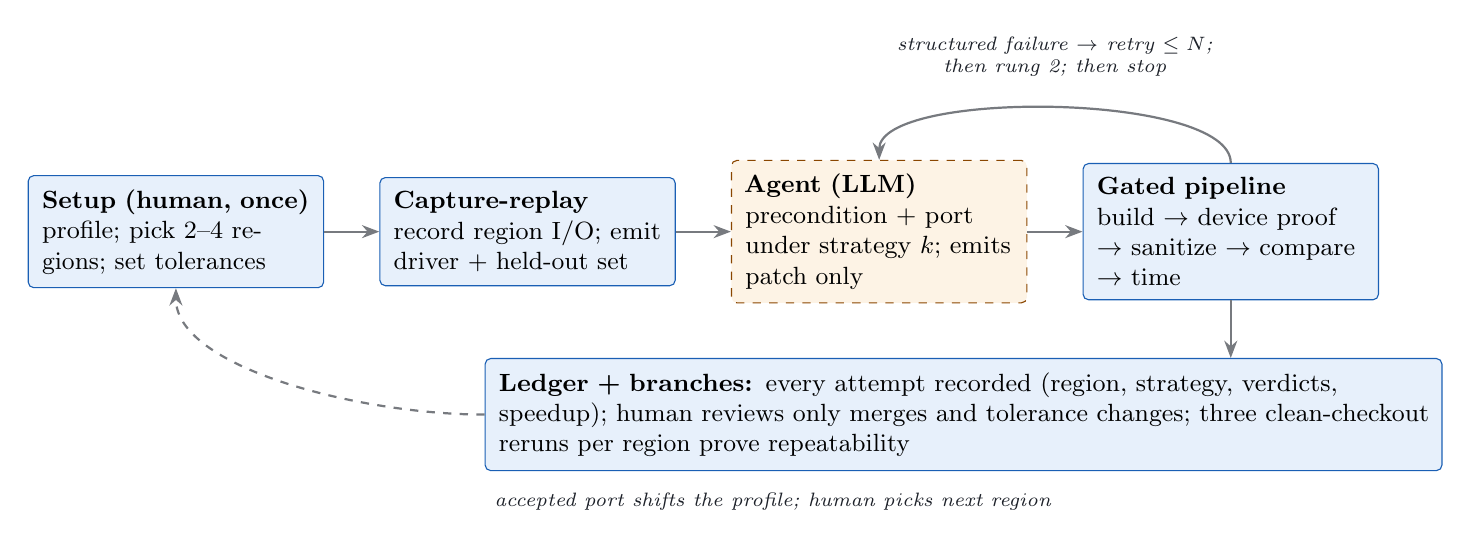
\begin{tikzpicture}[
  node distance=5mm and 7mm,
  box/.style={draw=accent, fill=boxfill, rounded corners=2pt, align=left,
              font=\small, inner sep=5pt, text width=34mm},
  sto/.style={box, draw=warn, fill=stofill, dashed},
  wide/.style={box, text width=118mm},
  lbl/.style={font=\scriptsize\itshape, text=ink},
  arr/.style={-{Stealth[length=2.2mm]}, thick, draw=ink!60}
]
\node[box] (setup) {\textbf{Setup (human, once)}\\ profile; pick 2--4 regions; set tolerances};
\node[box, right=of setup] (capture) {\textbf{Capture-replay}\\ record region I/O; emit driver + held-out set};
\node[sto, right=of capture] (agent) {\textbf{Agent (LLM)}\\ precondition + port under strategy $k$; emits patch only};
\node[box, right=of agent] (gates) {\textbf{Gated pipeline}\\ build $\to$ device proof $\to$ sanitize $\to$ compare $\to$ time};
\node[wide, below=8mm of $(capture.south)!0.62!(gates.south)$] (ledger)
  {\textbf{Ledger + branches:} every attempt recorded (region, strategy, verdicts, speedup); human reviews only merges and tolerance changes; three clean-checkout reruns per region prove repeatability};
\draw[arr] (setup) -- (capture);
\draw[arr] (capture) -- (agent);
\draw[arr] (agent) -- (gates);
\draw[arr] (gates.north) .. controls +(0,9mm) and +(0,9mm) .. (agent.north)
  node[lbl, above=9.5mm of $(agent.north)!0.5!(gates.north)$, align=center]
  {structured failure $\to$ retry $\le N$;\\ then rung 2; then stop};
\draw[arr] (gates.south) -- (gates.south |- ledger.north);
\draw[arr, dashed] (ledger.west) .. controls +(-16mm,0) and +(0,-10mm) .. (setup.south);
\node[lbl, below=1.5mm of ledger.south west, anchor=north west]
  {accepted port shifts the profile; human picks next region};
\end{tikzpicture}
\caption{The skateboard loop. The agent is the only stochastic component and touches nothing but its patch. Oracles and captured data are read-only to it. The outer loop (which region next) is human; the inner loop (make one region's port pass the gates) is autonomous and bounded.}
\end{figure}

Two deliberate simplifications inside the loop deserve a note. \emph{Candidate selection is human}: with one code, an engineer reading one profile picks the two to four demonstration regions in an afternoon, and we choose regions dominated by plain arrays and clean loop nests --- deferring derived types with allocatable components, which are the hard case for any state-capture tool. This is scope control, not evasion, and we say so in the report. \emph{Preconditioning is agent-proposed but conservatively validated}: the agent performs the de-\texttt{COMMON}-ing and \texttt{intent} annotation for its region as ordinary patches, the full existing test suite must pass after each preconditioning patch on the CPU path, and these patches get human review at merge like any other. The compiler-grade transform library from the full design is deferred, traded for region choice and suite coverage.

\section{Human touchpoints}

Exactly four, all logged: (1) initial region selection and tolerance sign-off; (2) review of any proposal to change a tolerance or accept a semantic difference the comparator surfaces --- expected rarely, and valuable when it happens, since it usually means the port exposed a latent defect such as argument aliasing or an uninitialized variable; (3) merge review per accepted port; (4) a go/no-go per region when the agent exhausts its ladder and caps. Everything else --- generation, repair against compiler errors, comparator discrepancies, and profiler feedback --- runs unattended. The report can then say: $M$ regions ported, $N$ total human interventions of these four kinds, everything else autonomous, with the ledger as evidence.

\section{What was cut, and what the cut costs}

Table~\ref{tab:cuts} lists every full-design component that the skateboard drops or substitutes, the consequence of the cut, and the condition under which it should be restored --- so the three-month artifact reads as the first increment of the full design rather than a different design.

\begin{table}[htbp]
\centering\small
\begin{tabular}{@{}p{0.26\textwidth}p{0.2\textwidth}p{0.46\textwidth}@{}}
\toprule
\textbf{Full-design component} & \textbf{Disposition} & \textbf{Cost, and when to restore} \\
\midrule
Planner (ranked regions, predicted ceilings) & Human, once & None for 2--4 regions. Restore when porting whole codes or many codes. \\
Deterministic preconditioner & Agent + suite + review & Slower, more review load. Restore (Flang/PSyclone-based) at scale, where LLM per-line error rates bite. \\
Multi-strategy ensemble & Two-rung ladder, sequential & May miss the best variant per region. Restore when GPU budget allows parallel strategy runs. \\
Provenance store (MVIR-like) & Git branches + CSV ledger & Adequate for one campaign. Restore for multi-code auditability. \\
Roofline service & Back-of-envelope, once & Weaker ``gap to ceiling'' attribution. Restore for tuning-heavy work. \\
Compiler/vendor matrix & One toolchain, one GPU & No portability claim. Restore before any multi-platform commitment. \\
Prompt optimization; model plurality & One model, versioned prompts & Possibly leaving quality on the table. Cheap to add later behind the same interface. \\
Evaluation battery (B01 analogue) & The code is the battery & No cross-code generality claim. Build the battery if this becomes a program. \\
\bottomrule
\end{tabular}
\caption{Everything cut is throughput or scale. Nothing cut weakens the correct/effective/repeatable evidence for the demonstrated regions --- but the demonstration claims exactly those regions, on exactly one platform, and the report should say so plainly.}
\label{tab:cuts}
\end{table}

\section{Three-month plan and the evidence pack}

\textbf{Month 1 --- oracles before agents.} Reproducible containerized build and CI on the existing test suite; profile on representative datasets; select regions and calibrate tolerances (human touchpoint 1); build the capture-replay generator and comparator for region~1; run the na\"ive \texttt{-stdpar} baseline and the honest multicore CPU baseline. Milestone: replay driver for region~1 passes against the CPU code under the tolerance policy, from a clean checkout, in CI. If month~1 slips, the schedule slips --- nothing downstream is real without this.

\textbf{Month 2 --- one region, fully assured.} Stand up the gated pipeline and the bounded agent loop; port region~1; iterate on structured feedback plumbing (this is where TRACTOR says the leverage is); first clean-checkout rerun. Milestone: region~1 accepted through all gates with a measured end-to-end speedup, and one rerun reproducing it.

\textbf{Month 3 --- breadth and the repeatability numbers.} Regions 2--3 (and 4 if cheap); three clean-checkout reruns per region; assemble the evidence pack; write the report, including the personal-versus-professional framing of Section~1.

The evidence pack is the point of the exercise, so we name its contents now: the tolerance policy with its calibration data; per-region comparator reports on visible and held-out sets; device-execution traces; sanitizer logs; the baseline-versus-port timing distributions; the ledger with intervention counts; and the rerun variance table. Every sentence of the final report's claims should trace to an artifact in this pack --- that traceability, more than any single speedup number, is what distinguishes the engineering-organization mode of AI use from the personal one.

\textbf{Principal risks.} (1) Capture-replay engineering exceeds estimates for the chosen regions --- mitigated by region selection (plain arrays first) and by the month-1 milestone acting as an early warning. (2) The na\"ive baseline wins on our regions --- then the demonstration reframes, honestly and still favorably, as ``AI verified and hardened the cheap port and proved where effort is unnecessary''; the assurance machinery is the deliverable either way. (3) GPU node availability and driver churn --- pin everything in month~1 and keep exclusive access for measurement runs. (4) The existing test suite is weaker than assumed, undermining preconditioning validation --- detected in month~1 by coverage measurement; the fallback is narrowing regions to code the replay tests themselves cover.

\end{document}
